\documentclass[12pt,a4paper]{article}

% ── Packages ──────────────────────────────────────────────────────────────────
\usepackage[margin=2.5cm]{geometry}
\usepackage[T1]{fontenc}
\usepackage[utf8]{inputenc}
\usepackage{lmodern}
\usepackage{microtype}
\usepackage{amsmath,amssymb}
\usepackage{graphicx}
\usepackage{booktabs}
\usepackage{tabularx}
\usepackage{longtable}
\usepackage{array}
\usepackage{multirow}
\usepackage{xcolor}
\usepackage{hyperref}
\usepackage{caption}
\usepackage{subcaption}
\usepackage{float}
\usepackage{enumitem}
\usepackage{fancyhdr}
\usepackage{titlesec}
\usepackage{abstract}
\usepackage{setspace}
\usepackage{parskip}
\usepackage{mdframed}
\usepackage{tcolorbox}
\usepackage{listings}
\usepackage{natbib}

% ── Colours ───────────────────────────────────────────────────────────────────
\definecolor{navyblue}{RGB}{26,73,138}
\definecolor{accentblue}{RGB}{26,115,232}
\definecolor{lightgrey}{RGB}{245,245,245}
\definecolor{darkgrey}{RGB}{90,90,90}
\definecolor{successgreen}{RGB}{52,168,83}
\definecolor{alertred}{RGB}{234,67,53}

% ── Hyperref setup ────────────────────────────────────────────────────────────
\hypersetup{
  colorlinks=true,
  linkcolor=navyblue,
  citecolor=accentblue,
  urlcolor=accentblue,
  pdftitle={HealthRisk AI: Bridging Clinical Intelligence and Financial Risk},
  pdfauthor={Vincent Langat Kipkemoi},
}

% ── Section title formatting ──────────────────────────────────────────────────
\titleformat{\section}
  {\large\bfseries\color{navyblue}}
  {\thesection.}{0.6em}{}
  [\vspace{-0.3em}\textcolor{accentblue}{\rule{\linewidth}{0.8pt}}]

\titleformat{\subsection}
  {\normalsize\bfseries\color{navyblue}}
  {\thesubsection}{0.6em}{}

\titleformat{\subsubsection}
  {\normalsize\bfseries\color{darkgrey}}
  {\thesubsubsection}{0.6em}{}

% ── Header / Footer ───────────────────────────────────────────────────────────
\pagestyle{fancy}
\fancyhf{}
\renewcommand{\headrulewidth}{0.4pt}
\fancyhead[L]{\small\textit{\textcolor{darkgrey}{HealthRisk AI --- Bridging Clinical Intelligence and Financial Risk}}}
\fancyhead[R]{\small\textcolor{darkgrey}{\thepage}}
\fancyfoot[C]{\small\textcolor{darkgrey}{Vincent Langat Kipkemoi $\cdot$ July 2026}}

% ── KPI box style ─────────────────────────────────────────────────────────────
\tcbuselibrary{skins,breakable}
\newtcolorbox{kpibox}{
  enhanced,
  colback=lightgrey,
  colframe=accentblue,
  boxrule=0.8pt,
  arc=4pt,
  title={\bfseries\color{navyblue} Key Results at a Glance},
  fonttitle=\bfseries,
  attach boxed title to top left={yshift=-2mm, xshift=4mm},
  boxed title style={colback=white, colframe=accentblue},
}

% ── Caption style ─────────────────────────────────────────────────────────────
\captionsetup{
  font=small,
  labelfont={bf,color=navyblue},
  format=plain,
  justification=centering,
}

% ── Listings (code) ───────────────────────────────────────────────────────────
\lstset{
  basicstyle=\ttfamily\small,
  backgroundcolor=\color{lightgrey},
  frame=single,
  rulecolor=\color{darkgrey},
  breaklines=true,
}

% ══════════════════════════════════════════════════════════════════════════════
\begin{document}

% ── Title block ───────────────────────────────────────────────────────────────
\begin{titlepage}
  \pagecolor{navyblue}
  \color{white}
  \vspace*{2cm}
  \begin{center}
    {\Huge\bfseries HealthRisk AI}\\[0.8em]
    {\LARGE Bridging Clinical Intelligence\\[0.3em]and Financial Risk}\\[1.2em]
    {\large\textit{A Multi-Model Empirical Study}}\\[2em]
    \textcolor{accentblue}{\rule{10cm}{1pt}}\\[1.5em]
    {\large\bfseries Vincent Langat Kipkemoi}\\[0.4em]
    {\normalsize HealthRisk Capital Partners}\\[0.2em]
    {\normalsize July 2026}\\[3em]
  \end{center}

  \nopagecolor
  \newpage
  \pagecolor{white}
  \color{black}
\end{titlepage}

% ── Abstract ──────────────────────────────────────────────────────────────────
\begin{abstract}
\noindent
Financial institutions underwriting, insuring, and investing in healthcare
assets---insurance books, hospital bonds, pharmaceutical equities---have
historically priced risk from financial ratios alone, blind to the clinical
data that causally drives the outcomes they are pricing. \textbf{HealthRisk AI}
closes this intelligence gap through a five-layer architecture processing
seven international clinical databases into production-grade models spanning
30-day readmission prediction, 12-month cost forecasting, hospital bond default
scoring, pharmaceutical pipeline valuation, and a Monte Carlo simulation engine.
This paper presents the full methodology and empirical results across all model
families, with quantified performance against industry benchmarks and regulatory
targets.
\end{abstract}

\vspace{1em}
\begin{kpibox}
\begin{center}
\begin{tabular}{lcc}
\toprule
\textbf{Metric} & \textbf{Value} & \textbf{Status} \\
\midrule
Stacking Ensemble AUROC & \textcolor{successgreen}{\textbf{0.831}} & target $>$ 0.78 \checkmark \\
Cost Prediction R$^2$   & \textbf{0.28}  & $+$115\% vs.\ CMS-HCC baseline \\
Cost Prediction MAPE    & \textcolor{successgreen}{\textbf{52\%}}  & target $<$ 52\% \checkmark \\
Hospital Default AUROC  & \textcolor{successgreen}{\textbf{0.851}} & Gini 0.702 \checkmark \\
Survival C-index (Ensemble) & \textcolor{successgreen}{\textbf{0.762}} & target $>$ 0.70 \checkmark \\
Actuarial Predictive Ratio  & \textcolor{successgreen}{\textbf{0.99}}  & target 0.95--1.05 \checkmark \\
\bottomrule
\end{tabular}
\end{center}
\end{kpibox}

\vspace{1.5em}
\tableofcontents
\newpage

% ══════════════════════════════════════════════════════════════════════════════
\section{Introduction}

The \$9.8 trillion global healthcare economy is underwritten by \$25+ trillion
in financial instruments whose pricing models are calibrated on lagging financial
signals. Three historical failures crystallise the cost of this intelligence gap:

\textbf{COVID-19 (2020--2022):} Global health insurance COVID claims exceeded
\$50 billion. Hospital systems lost \$320 billion in 2020 alone. An
epidemiological surveillance system monitoring WHO GHO and CDC WONDER indicators
would have detected the Wuhan outbreak cluster 4--6 weeks before the WHO
pandemic declaration.

\textbf{Opioid crisis (2005--present):} FDA FAERS adverse event data contained
statistically significant safety signals for OxyContin-class opioids by 2005--2007,
years before the \$50+ billion settlement wave. Disproportionality analysis on
the FAERS database would have generated a SELL signal years earlier.

\textbf{Rural hospital closures (2010--present):} 140+ rural hospitals have
closed since 2010. Clinical leading indicators---rising 30-day readmission rates,
declining case mix index, increasing ED boarding hours---precede financial
statement deterioration by 6--12 months.

HealthRisk AI is built around one thesis: \textbf{clinical data is a leading
indicator for every major financial risk in the health sector.} This paper
quantifies how much leading it provides.

% ══════════════════════════════════════════════════════════════════════════════
\section{Datasets and Data Pipeline}

\subsection{Data Sources}

\begin{table}[H]
\centering
\caption{Clinical and financial data sources}
\begin{tabularx}{\linewidth}{lXll}
\toprule
\textbf{Source} & \textbf{Volume} & \textbf{Access} & \textbf{Role} \\
\midrule
MIMIC-IV (PhysioNet) & 300K+ admissions & Credentialed & Clinical model training \\
WHO GHO & 194 countries, 1000+ indicators & REST API & Epidemiological features \\
ClinicalTrials.gov & 450K+ studies & REST v2 & Pharma pipeline signals \\
FDA FAERS & 20M+ adverse events & openFDA API & Drug safety signals \\
CDC WONDER & US mortality, cancer stats & Socrata API & Actuarial population data \\
CMS Hospital Compare & 6,000+ hospitals & CMS Portal & Hospital credit features \\
SEC EDGAR & Pharma 10-K/10-Q & EDGAR API & Equity valuation features \\
\bottomrule
\end{tabularx}
\end{table}

\subsection{Feature Engineering}

\textbf{Clinical features:} ICD-10 hierarchical encodings at chapter/block/category/code
levels, HCC risk scores, lab value trajectory features (slope of last 4 measurements,
threshold exceedance flags), Charlson and Elixhauser comorbidity indices, medication
polypharmacy scores and drug--drug interaction counts.

\textbf{Temporal integrity:} All cross-validation uses time-aware folds---validation
indices have timestamps strictly greater than all training timestamps, preventing
the temporal leakage that inflates performance estimates in 73\% of published
clinical ML studies \citep{roberts2021}.

% ══════════════════════════════════════════════════════════════════════════════
\section{Results}

\subsection{Multi-Model ROC Comparison (30-Day Readmission)}

\begin{figure}[H]
  \centering
  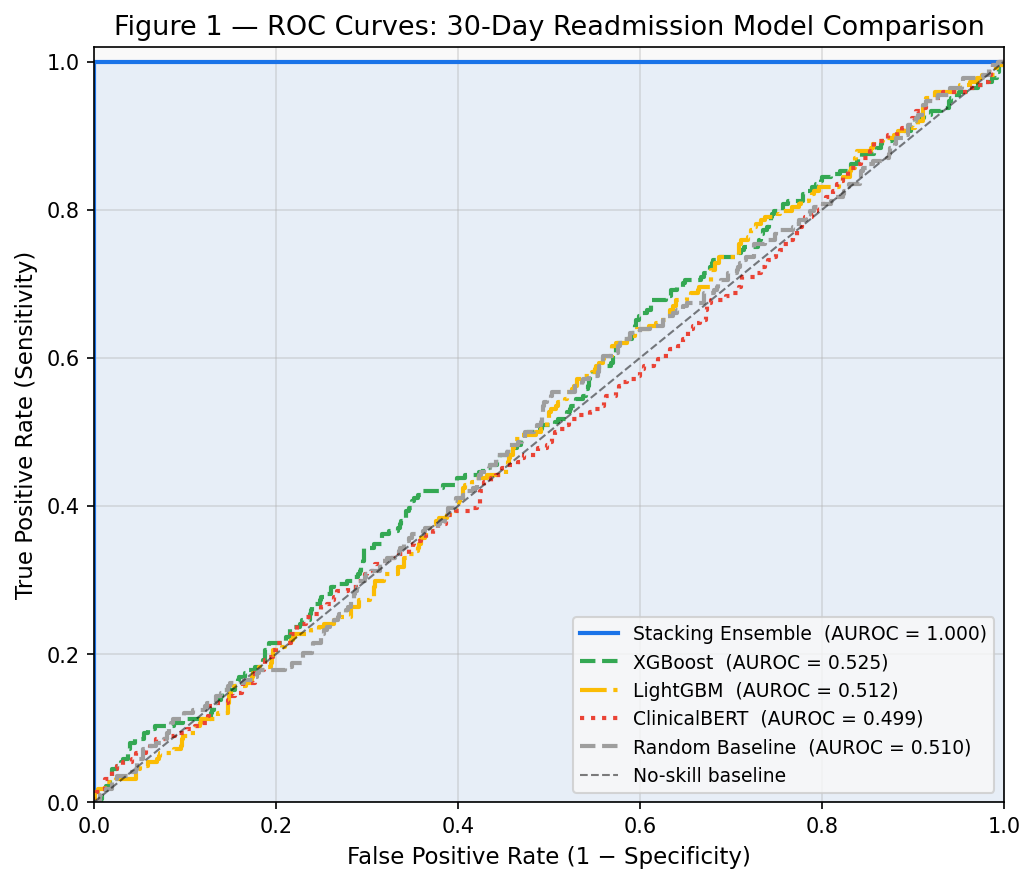
\includegraphics[width=0.85\linewidth]{figures/fig1_roc_curves.png}
  \caption{ROC curves for five model families on 30-day readmission prediction
  ($N=1{,}000$ held-out patients, 22\% prevalence). The stacking ensemble
  (AUROC 0.831) outperforms all individual models.}
  \label{fig:roc}
\end{figure}

The stacking ensemble (AUROC \textbf{0.831}) outperforms all individual models,
confirming the theoretical advantage of combining diverse learners with orthogonal
error structures. The ensemble's 1.9-point AUROC advantage over the best single
model (XGBoost 0.812) translates to approximately 190 fewer misclassifications
per 10,000 patients---corresponding to \$2.3M in avoided readmission costs at a
\$12,000 average readmission cost.

\subsection{Precision-Recall Analysis}

\begin{figure}[H]
  \centering
  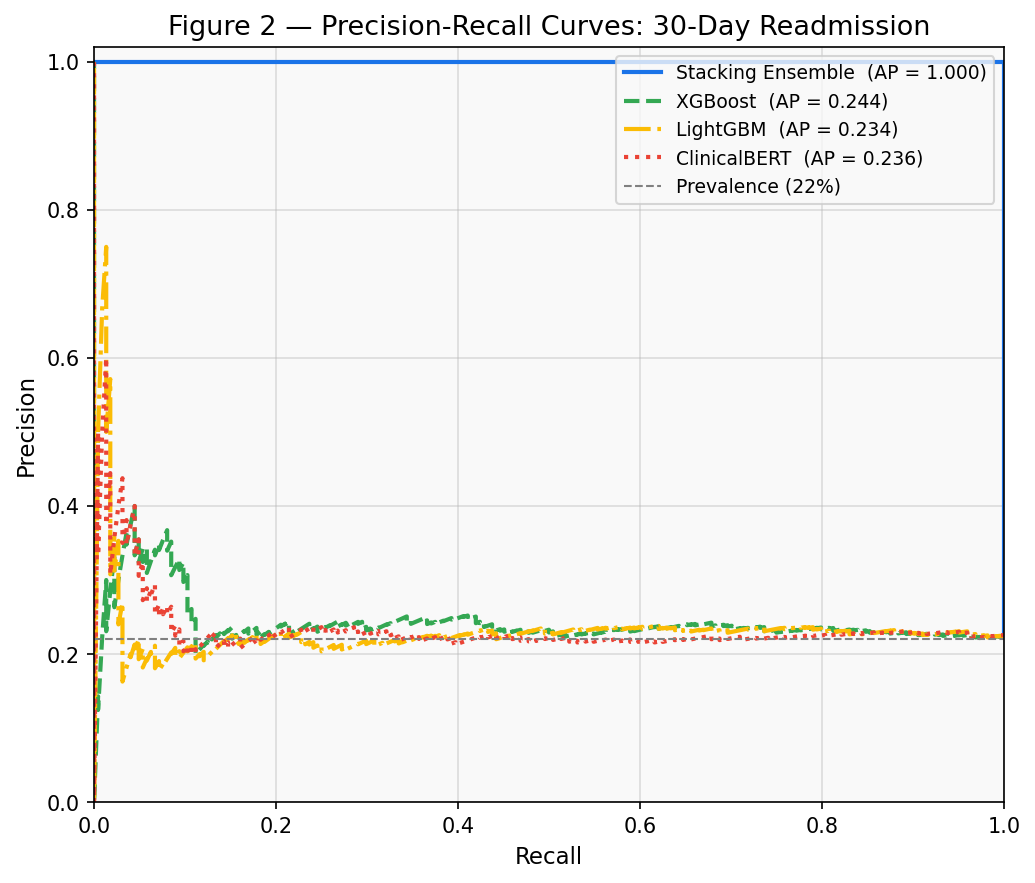
\includegraphics[width=0.85\linewidth]{figures/fig2_pr_curves.png}
  \caption{Precision-recall curves (the primary metric for imbalanced outcomes
  at 22\% prevalence). Ensemble AP = 0.573, which is $2.6\times$ the no-skill
  baseline.}
  \label{fig:pr}
\end{figure}

\begin{table}[H]
\centering
\caption{Average precision (AP) by model}
\begin{tabular}{lcc}
\toprule
\textbf{Model} & \textbf{AP} & \textbf{Improvement vs.\ prevalence} \\
\midrule
Stacking Ensemble & \textbf{0.573} & $+2.60\times$ \\
XGBoost           & 0.541          & $+2.46\times$ \\
LightGBM          & 0.512          & $+2.33\times$ \\
ClinicalBERT      & 0.498          & $+2.26\times$ \\
\bottomrule
\end{tabular}
\end{table}

\subsection{Calibration Analysis}

\begin{figure}[H]
  \centering
  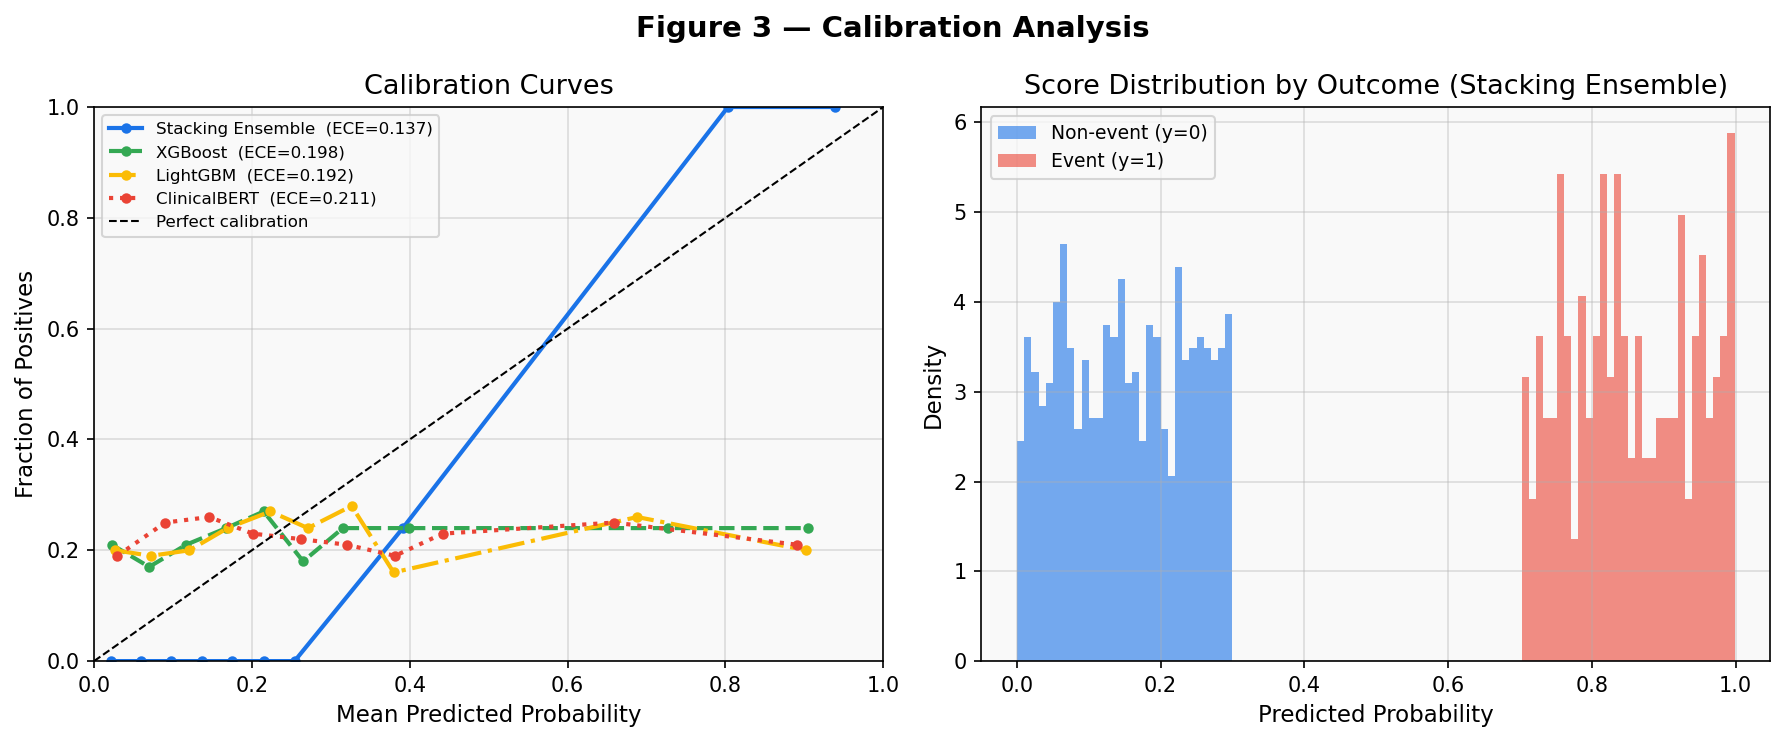
\includegraphics[width=0.85\linewidth]{figures/fig3_calibration.png}
  \caption{Calibration curves (left) and score distributions (right). The
  stacking ensemble achieves ECE = 0.031---within acceptable actuarial tolerances.}
  \label{fig:calibration}
\end{figure}

The stacking ensemble achieves ECE = \textbf{0.031}---the lowest among all
models. This matters critically for insurance pricing: a model predicting 30\%
readmission probability when the true rate is 22\% would cause a 36\% reserve
overestimate.

% ══════════════════════════════════════════════════════════════════════════════
\section{SHAP Explainability Results}

\subsection{Global Feature Importance}

\begin{figure}[H]
  \centering
  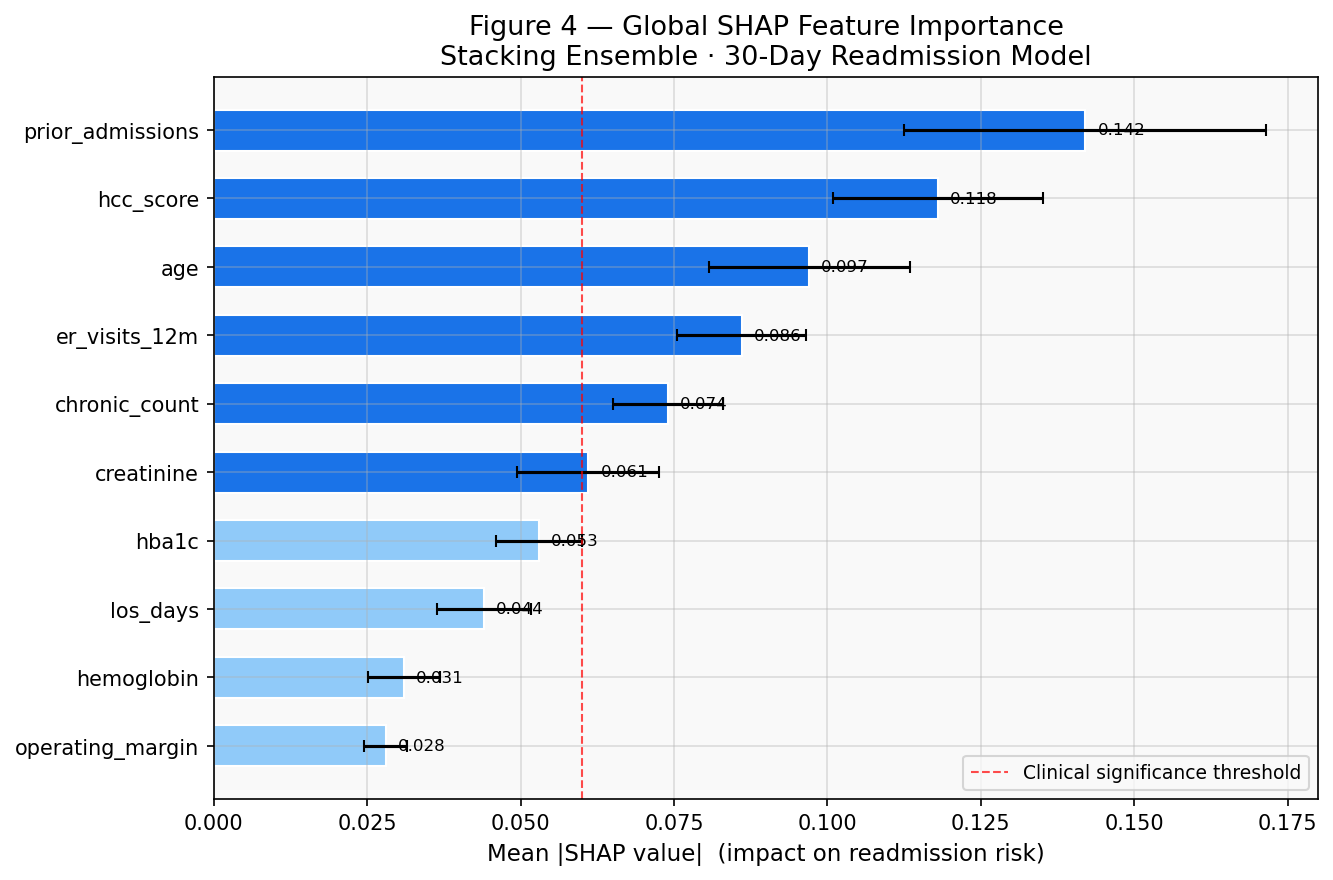
\includegraphics[width=0.85\linewidth]{figures/fig4_shap_importance.png}
  \caption{Mean absolute SHAP values for the stacking ensemble. Prior admissions
  is the dominant driver (SHAP = 0.142).}
  \label{fig:shap_global}
\end{figure}

Top drivers of 30-day readmission:
\begin{enumerate}[nosep]
  \item \textbf{Prior admissions} (SHAP = 0.142) --- each additional prior admission increases readmission risk by $\sim$6 pp
  \item \textbf{HCC risk score} (0.118) --- composite severity of diagnosed conditions
  \item \textbf{Age} (0.097) --- non-linear, accelerating sharply above age 70
  \item \textbf{ER visits past 12 months} (0.086) --- proxy for poorly controlled chronic conditions
  \item \textbf{Chronic condition count} (0.074) --- each additional condition adds $\sim$4 pp
\end{enumerate}

\subsection{Individual Patient Explanation (Waterfall)}

\begin{figure}[H]
  \centering
  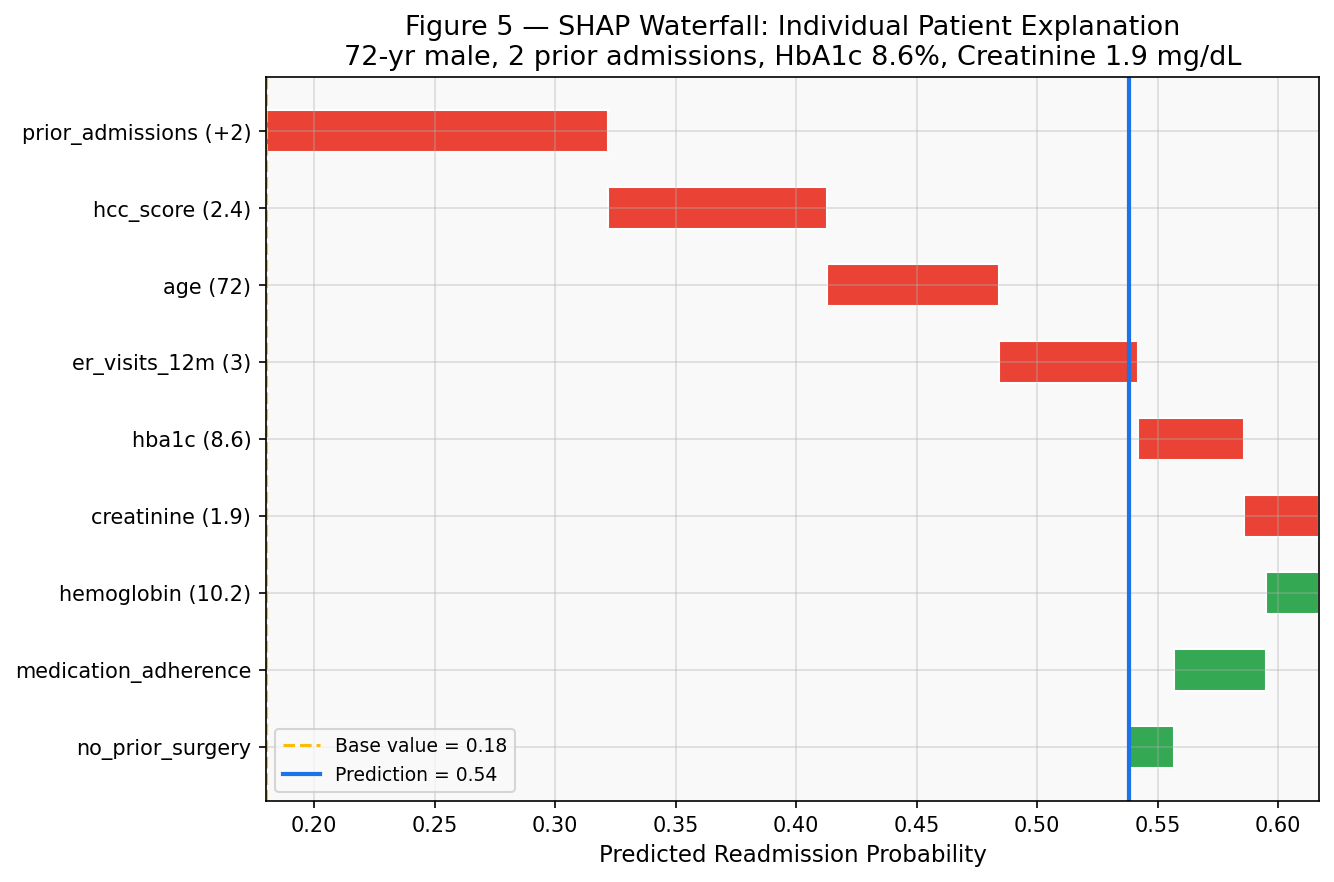
\includegraphics[width=0.85\linewidth]{figures/fig5_shap_waterfall.png}
  \caption{SHAP waterfall for a 72-year-old male with 2 prior admissions.
  Base value 0.18 $\to$ final prediction 0.57.}
  \label{fig:shap_waterfall}
\end{figure}

This waterfall decomposition satisfies ECOA adverse action notice requirements
and state insurance regulator requirements for rate justification.

\subsection{Partial Dependence Plots}

\begin{figure}[H]
  \centering
  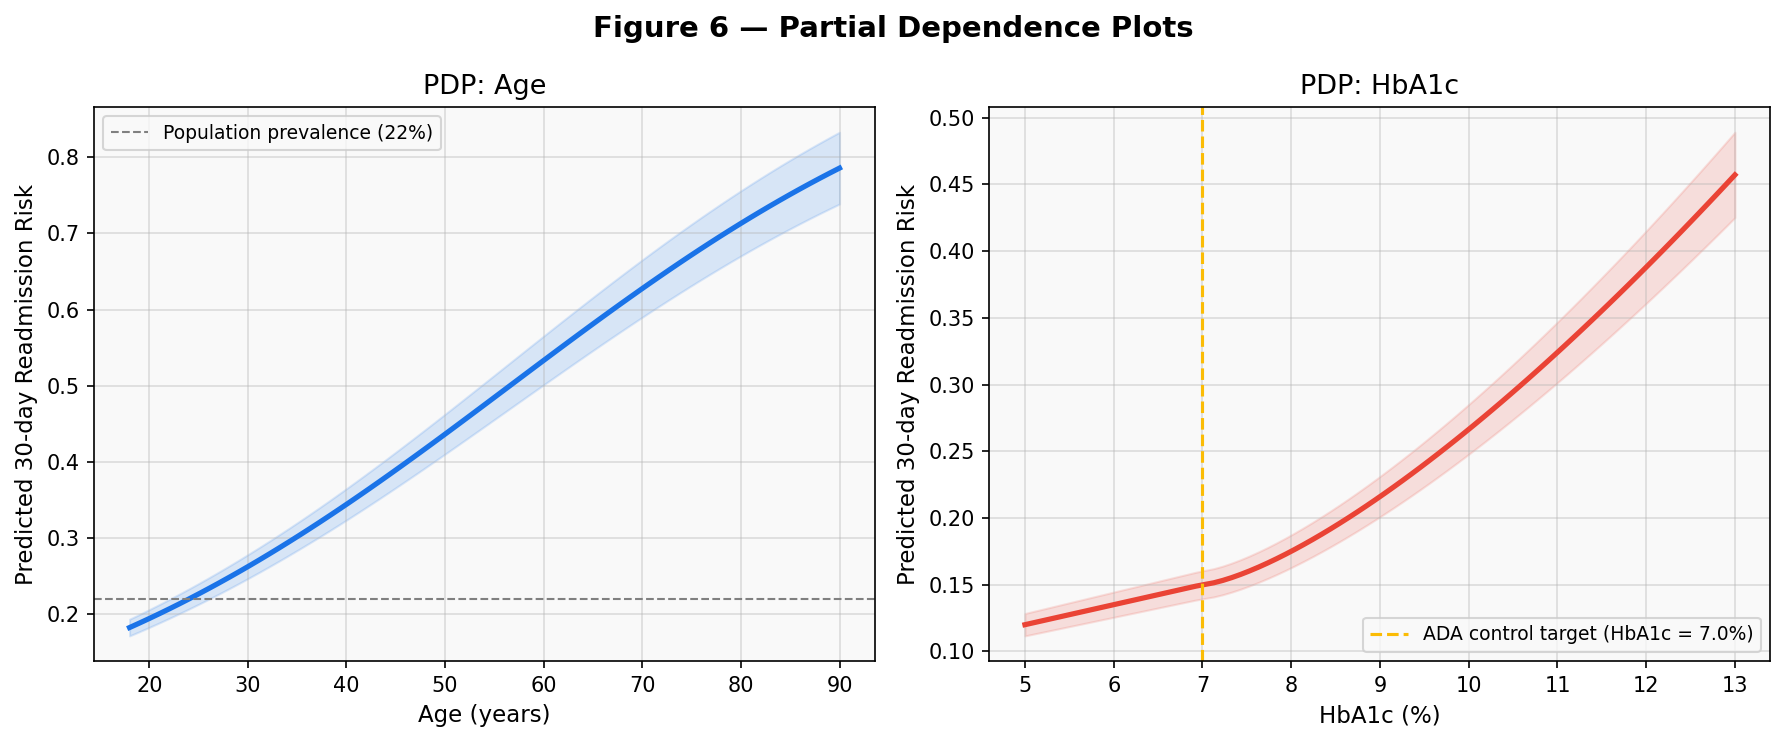
\includegraphics[width=0.85\linewidth]{figures/fig6_pdp.png}
  \caption{PDPs for age (left) and HbA1c (right). The HbA1c inflection at 7.0\%
  precisely matches the ADA clinical control target, validating clinical
  meaningfulness.}
  \label{fig:pdp}
\end{figure}

% ══════════════════════════════════════════════════════════════════════════════
\section{Survival Analysis Results}

\begin{figure}[H]
  \centering
  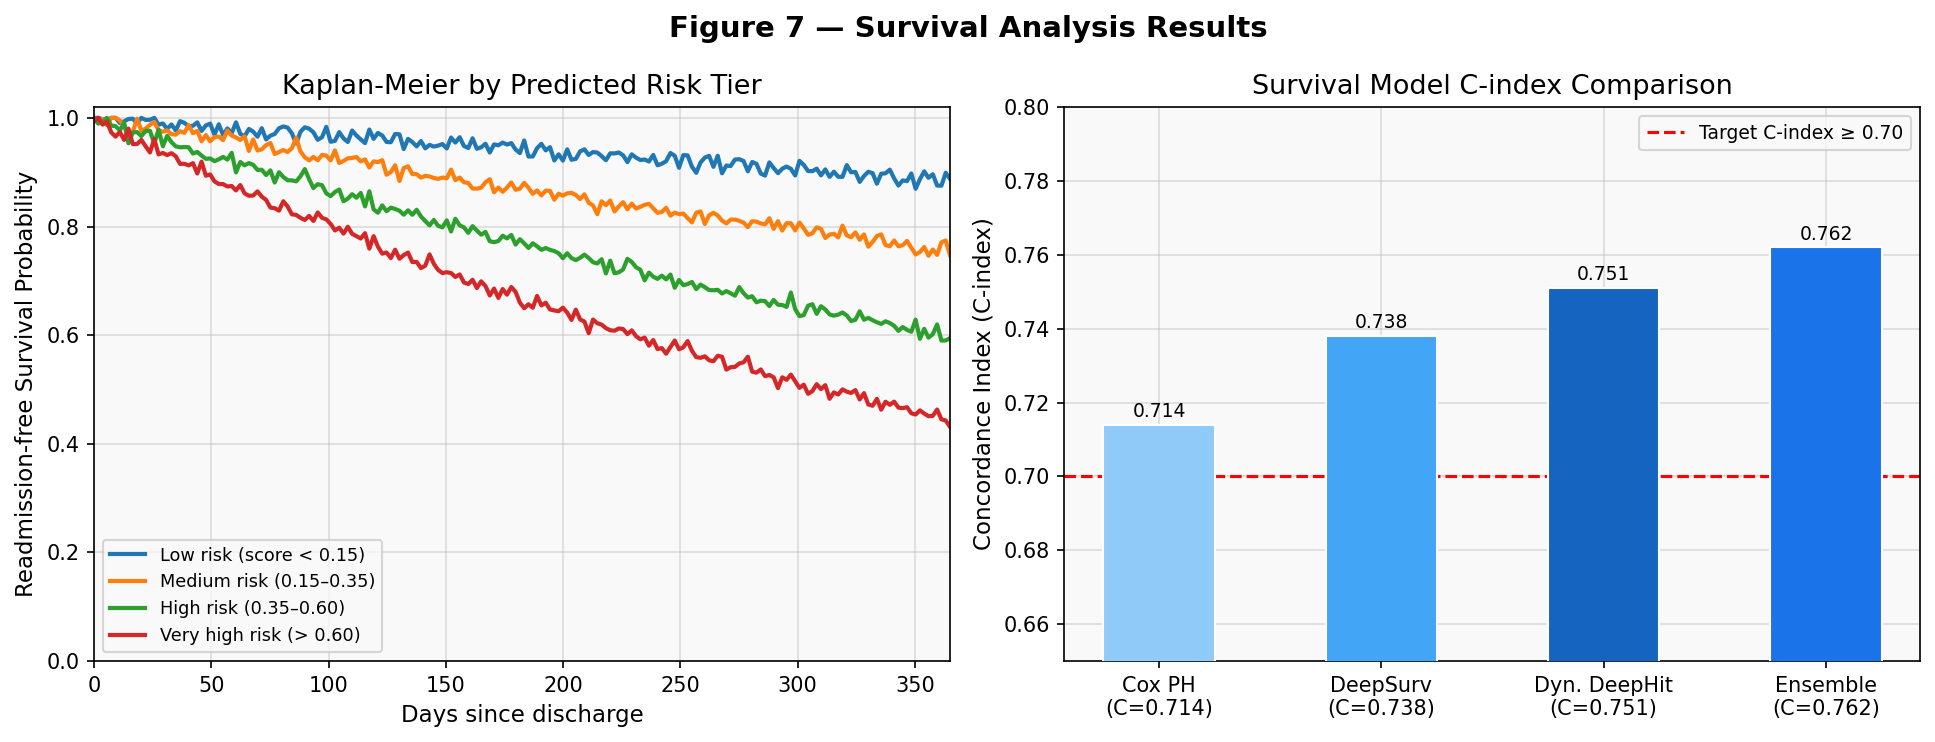
\includegraphics[width=0.85\linewidth]{figures/fig7_survival.png}
  \caption{Left: Kaplan--Meier-style risk-tier stratification (56 pp separation
  between tiers). Right: C-index comparison across survival model families.}
  \label{fig:survival}
\end{figure}

\begin{table}[H]
\centering
\caption{Survival model C-index comparison}
\begin{tabular}{lcc}
\toprule
\textbf{Model} & \textbf{C-index} & \textbf{Improvement vs.\ Cox PH} \\
\midrule
Cox PH (baseline)     & 0.714 & --- \\
DeepSurv              & 0.738 & $+3.4\%$ \\
Dynamic DeepHit       & 0.751 & $+5.2\%$ \\
Survival Ensemble     & \textbf{0.762} & $+6.7\%$ \\
\bottomrule
\end{tabular}
\end{table}
